\documentclass{article}
\usepackage{graphicx}
\usepackage[utf8]{inputenc}
\usepackage{amsmath, amssymb, latexsym}

\usepackage{pgfplots}
\usepackage{algorithm}
\usepackage[noend]{algpseudocode}
\usepackage{tikz}
\usepackage{nicefrac}
\pgfplotsset{every axis legend/.append style={
at={(0,0)},
anchor=north east}}
\usetikzlibrary{shapes,positioning,intersections,quotes}
\usetikzlibrary{arrows.meta,
                bending,
                intersections,
                quotes,
                shapes.geometric}
                
\definecolor{darkgreen}{rgb}{0.0, 0.6, 0.0}
\definecolor{darkred}{rgb}{0.7, 0.0, 0.0}
\makeatletter
\def\BState{\State\hskip-\ALG@thistlm}
\makeatother
\title{Week 2}
\begin{document}
  \pagenumbering{gobble}
  \maketitle
  \newpage
  \pagenumbering{arabic}

\section*{Linear Regression}
The previously described home price data example is an example of a supervised learning regression problem.
\subsection*{Notation (used throughout the course)}
\begin{itemize}
\item $m$ = number of training examples.
\item $x's$ = input variables / features.
\item $y's$ = output variable "target" variables.
\item $(x,y)$ - single training example.
\item $(x^i, y^j)$ - specific example (ith training example).
\end{itemize}

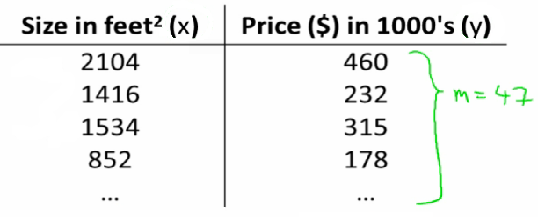
\includegraphics[width=0.8\textwidth]{resources/house_price_table}

\subsection*{With our training set defined - how do we used it?}
\begin{itemize}
\item Take training set.
\item Pass into a learning algorithm.
\item Algorithm outputs a function (h = hypothesis).
\item This function takes an input (e.g. size of new house).
\item Tries to output the estimated value of Y.
\end{itemize}

$$h_{\theta}(x) = \theta_0 + \theta_1x$$

\begin{itemize}
\item Y is a linear function of x!
\item $\theta_0$ is zero condition.
\item $\theta_1$ is gradient.
\end{itemize}

\subsection*{Cost function}
\begin{itemize}
\item We may use a cost function to determine how to fit the best straight line to our data.
\item We want to want to solve a minimization problem. Minimize $(h_{\theta}(x) - y)^2$.
\item Sum this over the training set.
\end{itemize}

$$J(\theta_0, \theta_1) = \frac{1}{2m} \sum_{m}^{i=1}(h_{\theta}(x^{(i)}) - y^{(i)})^2$$


\subsection*{Example}

For $ \theta_0 = 0$ we have:

$$h_{\theta}(x) = \theta_1x\quad and \quad J(\theta_1) = \frac{1}{2m} \sum_{m}^{i=1}(h_{\theta}(x^{(i)}) - y^{(i)})^2$$

Data:
\begin{itemize}
\item $\theta_1 = 1$ and $J(\theta_1)= 0$.
\item $\theta_1 = 0.5$ and $J(\theta_1)= 0.58$.
\item $\theta_1 = 0$ and $J(\theta_1)= 2.3$.
\end{itemize}

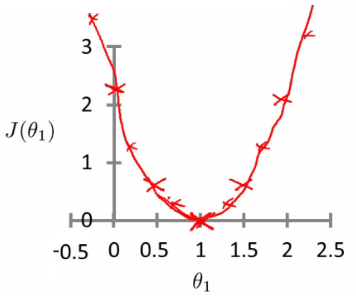
\includegraphics[width=0.7\textwidth]{resources/cost_function}

~\\
The optimization objective for the learning algorithm is find the value of $\theta_1$ which minimizes $J(\theta_1)$.
So, here $\theta_1 = 1$ is the best value for $\theta_1$.

\subsection*{A deeper insight into the cost function - simplified cost function}

The real cost function takes two variables as parameters! $J(\theta_0, \theta_1)$.

~\\We can now generates a 3D surface plot where axis are:

\begin{itemize}
\item $X = \theta_1$.
\item $Z = \theta_0$.
\item $Y = J(\theta_0,\theta_1)$.
\end{itemize}

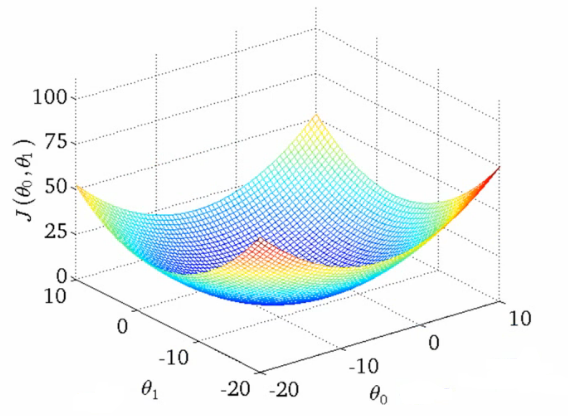
\includegraphics[width=0.8\textwidth]{resources/surface_cost_function}

The best hypothesis is at the bottom of the bowl.

~\\
Instead of a surface plot we can use a contour figures/plots.
\begin{itemize}
\item Set of ellipses in different colors.
\item Each colour is the same value of  $J(\theta_0,\theta_1)$, but obviously plot to different locations because $\theta_1$ and $\theta_0$ will vary.
\item Imagine a bowl shape function coming out of the screen so the middle is the concentric circles.
\end{itemize}

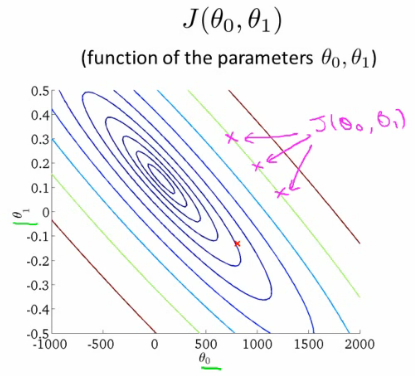
\includegraphics[width=0.6\textwidth]{resources/contour_cost_function}

The best hypothesis is located in the center of the contour plot.

\section*{Gradient descent algorithm}
\begin{itemize}
\item Begin with initial guesses, could be (0,0) or any other value.
\item Continually change values of $\theta_0$ and $theta_1$ to try to reduce  $J(\theta_0, \theta_1)$.
\item Continue until you reach a local minimum.
\item Reached minimum is determined by the starting point.
\end{itemize}

\begin{center}
    \large
    \textbf{Surface plot of gradient descent.}
	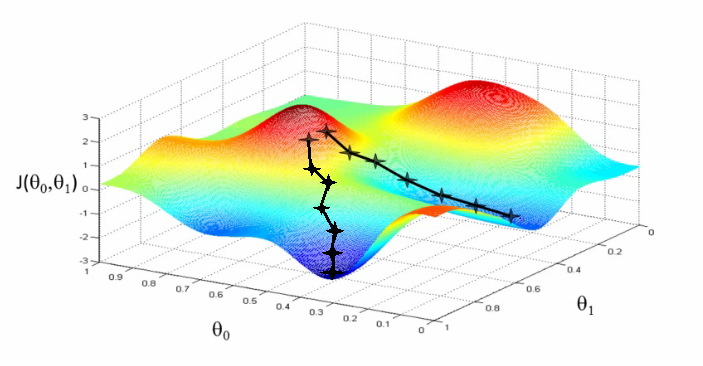
\includegraphics[width=\textwidth]{resources/gradient_descent}
\end{center}

 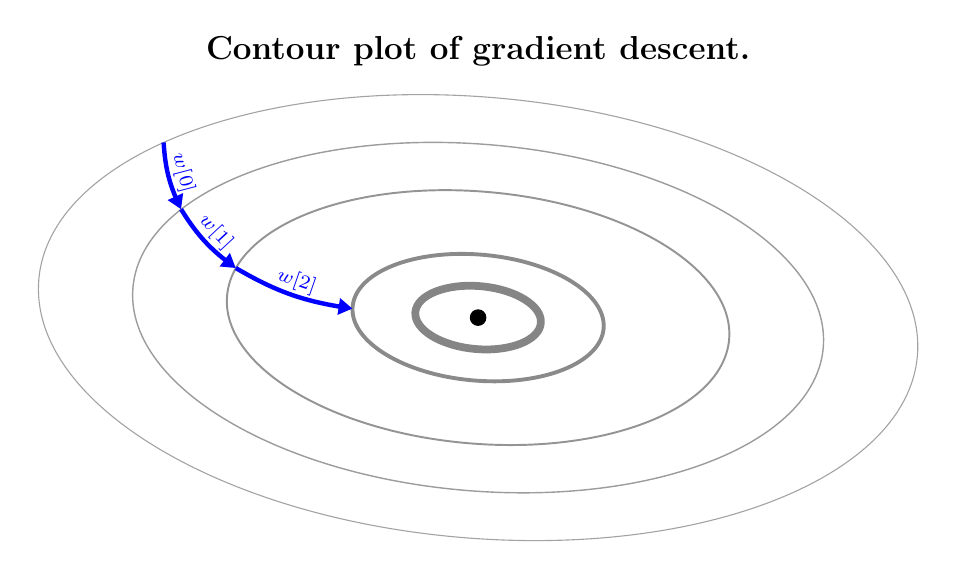
\begin{tikzpicture}[
every edge/.style = {draw, -{Triangle[angle=60:1pt 3,flex]},
                             bend right=11, blue,ultra thick},
every edge quotes/.style = {font=\scriptsize, inner sep=1pt, 
                            auto, sloped}
                            ]
\fill (0,0) circle[radius=3pt];
\path[name path=C] foreach \i in {4, 8, 16, 22, 28}
        {(0,0) circle[draw=red!\i, x radius=2*\i mm, y radius=\i mm, rotate=-5]};
\foreach \i in  {4, 8, 16, 22, 28}
    \draw[line width=11.2/\i, draw=white!\i!gray]
        (0,0) circle[x radius=2*\i mm, y radius=\i mm, rotate=-5];
\path[name path=V] (-4,2.4) .. controls + (0,-2) and + (-2,0) .. (0,0);
%
\draw [name intersections={of=C and V, sort by=C, name=A}]
        (A-5) edge ["${w[0]}$"] (A-4)
        (A-4) edge ["${w[1]}$"] (A-3)
        (A-3) edge ["${w[2]}$"] (A-2);
        \node[above,font=\large\bfseries] at (current bounding box.north) {Contour plot of gradient descent.};
    \end{tikzpicture}


\begin{algorithm}
\caption{Gradient Descent}\label{euclid}
\begin{algorithmic}[1]
\Large
\While {not converged}
\State $\theta_j := \theta_j - \alpha \frac{\partial}{\partial \theta_j} J(\theta_0, \theta_1)$.
\State $(for\ j = 1\ and\ j=0)$
\EndWhile
\end{algorithmic}
\end{algorithm}

\subsection*{Two key terms in the algorithm:}
\begin{itemize}
\item $\alpha$ term
\item Derivative term
\end{itemize}

\subsection*{Partial derivative vs. derivative}
\begin{itemize}
\item Use partial derivative when we have multiple variables but only derive with respect to one.
\item Use derivative when we are deriving with respect to all the variables.
\end{itemize}

\subsection*{Derivative says:}
\begin{itemize}
\item Let's look at the slope of the line by taking the tangent at the point.
\item As a result, going towards the minimum (down) will result in a negative derivative; nevertheless, alpha is always positive, thus $J(\theta_1)$ will be updated to a lower value.
\item Similarly, as we progress up a slope, we increase the value of $J(\theta_1)$.
\end{itemize}

\subsection*{$\alpha$ term}
\begin{itemize}
\item If it's too small, it takes too long to converge.
\item If it is too large, it may exceed the minimum and fail to converge.
\end{itemize}

\subsection*{When you get to a local minimum}
\begin{itemize}
\item Gradient of tangent/derivative is 0
\item So derivative term = 0
\item $\alpha \cdot 0 = 0$
\item So $\theta_1 = \theta_1 - 0$.
\item So $\theta_1$ remains the same.
\end{itemize}

\section*{Linear regression with gradient descent}

Apply gradient descent to minimize the squared error cost function $J(\theta_0, \theta_1)$.

$$\frac{\partial}{\partial \theta_j} J(\theta_0, \theta_1) = \frac{\partial}{\partial \theta_j} \frac{1}{2m} \sum_{i=1}^{m} (h_{\theta}(x^{(i)}) - y^{(i)})^2$$

$$= \frac{\partial}{\partial \theta_j} \frac{1}{2m} \sum_{i=1}^{m} (\theta_0 + \theta_1x^{(i)} - y^{(i)})^2$$

~\\
For each case, we must determine the partial derivative:

$$j=0:\frac{\partial}{\partial \theta_0} J(\theta_0, \theta_1)=\frac{\partial}{\partial \theta_j} \frac{1}{m} \sum_{i=1}^{m} (h_{\theta}(x^{(i)}) - y^{(i)})$$

$$j=1:\frac{\partial}{\partial \theta_1} J(\theta_0, \theta_1)=\frac{\partial}{\partial \theta_j} \frac{1}{m} \sum_{i=1}^{m} (h_{\theta}(x^{(i)}) - y^{(i)})x^{(i)}$$

~\\
The linear regression cost function is always a convex function - always has a single minimum. So gradient descent will always converge to global optima.

\section*{Two extension to the algorithm}

\subsection*{Normal equation for numeric solution}
\begin{itemize}
\item To solve the minimization problem we can solve it $[ min J(\theta_0, \theta_1) ]$ exactly using a numeric method which avoids the iterative approach used by gradient descent.
\item Normal equations method.
\item Can be much faster for some problems, but it much more complicated (will be covered in detail later).
\end{itemize}

\subsection*{We can learn with a larger number of features}
\begin{itemize}
\item e.g. with houses, Size, Age, Number bedrooms, Number floors...
\item Can't really plot in more than 3 dimensions.
\item Best way to get around with this is the notation of linear algebra (matrices and vectors).
\end{itemize}

\end{document}